\section{Background Research}\label{lit}
\subsection{Introduction}
This study aims to create a method of detecting incongruence in news articles. Before the implementation begins, it is essential to review the existing literature to give the study context.

This literature review begins by defining several different types of incongruence and specifies the bounds applicable to this study. 

It then goes on to evaluate several existing approaches, which are discussed to give a clearer picture of the field as it stands, and the gaps present in the research concerning incongruence detection. These sources are also analysed to gain insight into possible approaches to tackle the problem at hand.

Natural language processing (NLP) is then defined, and different features and approaches reviewed and discussed.

\subsection{Types of Incongruence}

In the scope of media, incongruence is a broad term that covers many different forms of deception and misleading information. \citeA{chesney2017} classifies three different types of incongruent news articles: clickbait, fake news, and sensationalism.

\paragraph{Clickbait}
\citeA{potthast2016} define clickbait as a kind of "web content [...] designed to entice its readers into clicking an accompanying link". Clickbait uses exaggerated language, outright fake information and can be accompanied by graphics designed to entice a reader. Figure \ref{fig:clickbait} shows an example of clickbait, sourced from a Natural Health website \footnote{\url{https://naturalon.com/}}.

\begin{figure}[ht!]
  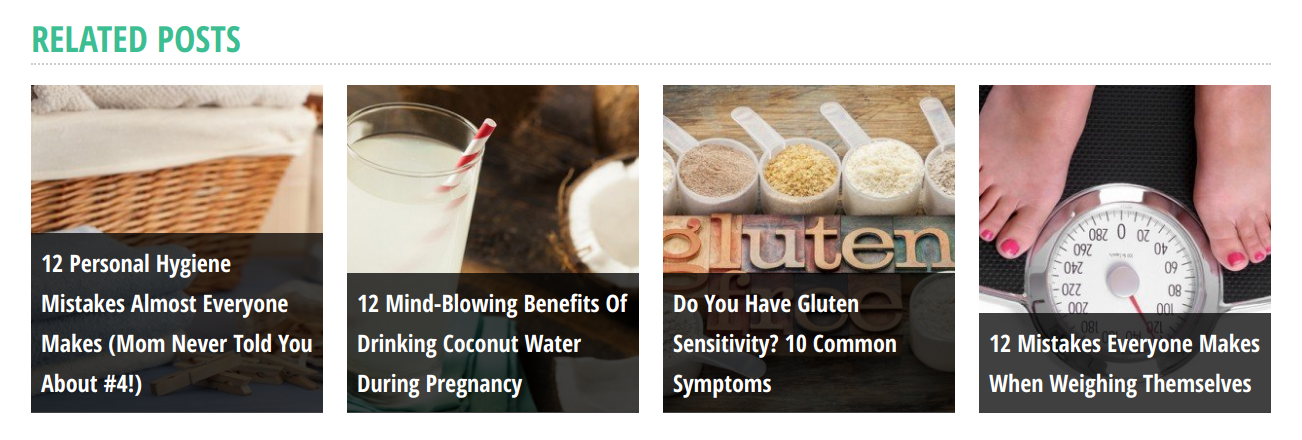
\includegraphics[width=\linewidth]{images/clickbait.png}
  \caption{Several clickbait articles in a 'chum box'}
  \label{fig:clickbait}
\end{figure}

\citeA{mahoney2015} terms a collection of clickbait stories as a 'chum boxes' - chum being dead fish used to bait other fish. \citeauthor{mahoney2015} goes on to examine how clickbait uses psychological methods to manipulate and how they can have an unconscious effect on an individual.

\paragraph{Fake News}
\citeA{allcott2017} defines fake news as "news articles that are intentionally and verifiably false, and could mislead readers". For example, a fake news conspiracy theory claimed that a pizzeria, Comet Ping Pong, in Washington ran a child sex ring in its basement. Figure \ref{fig:fakenews} shows a news article from 2016 from Your News Wire\footnote{\url{https://archive.is/YTk3n}} (now News Punch).


\begin{figure}[ht!]
  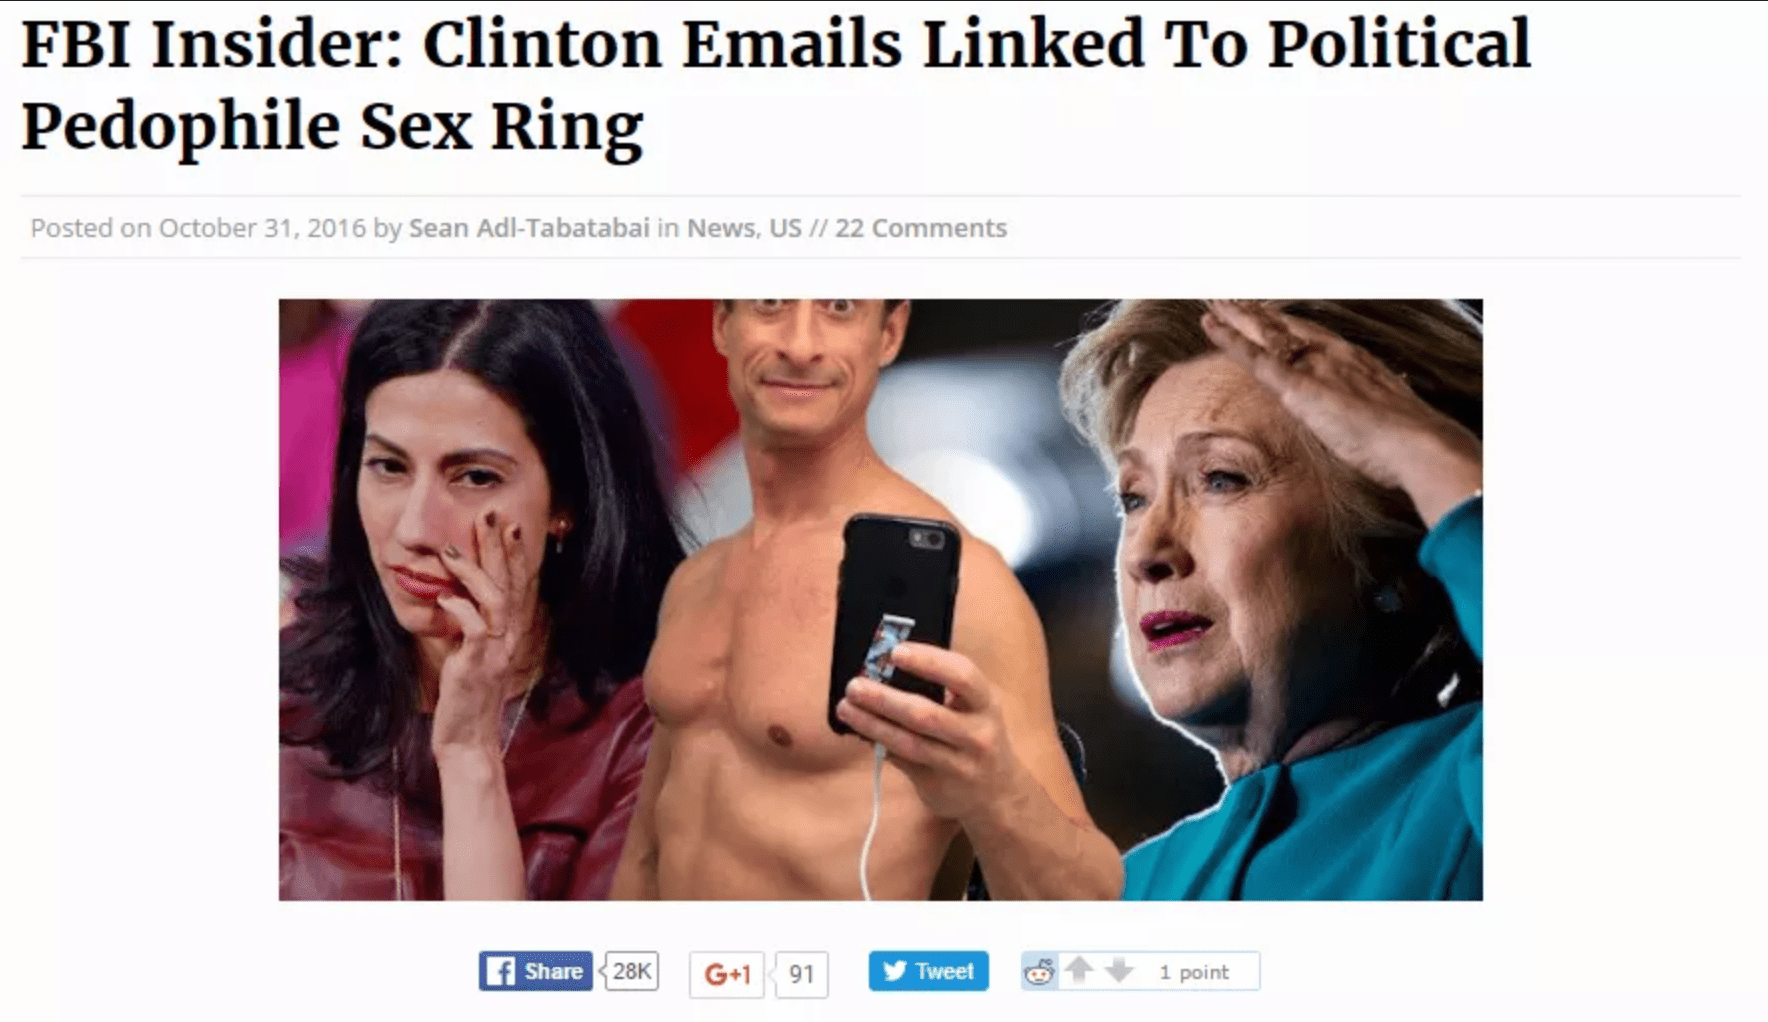
\includegraphics[width=\linewidth]{images/fakenews.png}
  \caption{A fake news story}
  \label{fig:fakenews}
\end{figure}


This conspiracy theory, perpetuated by fake news, lead to a man walking into the Comet Ping Pong pizzeria with an assault rifle and firing several shots. The restaurant's owner and staff also received several death threats \cite{lopez2016}.

\citeauthor{allcott2017} go further in their definition and give the following sub-categories for fake news: satire, parody, fabrication, manipulation, advertising and propaganda. While satire and parody's intention is not to deceive but to criticise, the other classifications have more subversive aims, such as misinforming people or gaining as many clicks as possible.

\paragraph{Sensationalism}
\citeA{molek2013} defines sensationalism as "a specific discourse strategy aimed at channeling audience's attention,  which may well be  resorted to by both popular and quality outlet". They suggest that media fails to provide important and valuable news, preferring superficial and quick-paced content.

Below are examples of sensationalised headlines sourced from The Sun:

\begin{itemize}
	\item DOOMSDAY DISEASE FEARS Terrorists could turn 'sniff and die' virus that kills victims in 24 hours into a BIO-WEAPON
	\item SPICE UP YOUR LIFE Chilli and ginger 'slash the risk of cancer – stopping tumours growing'
	\item JAB DEBATE As Melinda Messenger slams the HPV jab the parents of two teenagers blame their daughters' 'paralysis on vaccine'
	\item 'I KNOW WHO KILLED JONBENET' Juror from the JonBenet Ramsey case gives sensational interview revealing he 'knows who killed six-year-old'
	
\end{itemize}

These headlines use dramatic language ('slams', 'sensational', 'slash') to evoke a sense of urgency and excitement in the reader, urging them to click through to the rest of the article. Unlike clickbait headlines, information is not withheld but rather dramatised - while the aim is still to get as many clicks as possible; this is achieved through different means.

This sensationalism is intended to provoke and entertain, at times at the expense of accuracy \cite{chesney2017}. The below headline, again from The Sun, illustrates this well:

\begin{quote}
UK lockdown: March 29 rules loophole means you CAN go inside your pal or family’s home as restrictions ease \footnote{\url{https://www.thesun.co.uk/news/14453072/can-visit-garden-lockdown-eases-indoors-loo/}}
\end{quote}

This headline suggests that people will be able to socially gather inside someone else's house as a result of the ease of coronavirus restrictions. However, this is not the case; the article's body reveals that you can only enter a friend's house to use the toilet or if you're walking through to access an outdoor space such as a garden, and that meeting indoors is still banned.
 This example shows the danger of sensational headlines - by describing a deliberate, common-sense exception to legeslation as a loophole, readers may be under the false impression that it is acceptable to subvert restrictions and mix socially indoors.


\subsubsection{Project scope}
Fake news is not the focus of this project - by its nature, the entirety of a fake news article will be false, not just the headline. Therefore, to determine whether an article is fake, external sources would have to be consulted. Creating an algorithm for truth, while an open problem in computer science\footnote{\url{https://www.youtube.com/watch?v=leX541Dr2rU}}, is considered out of scope.

Instead, this study seeks to evaluate the extent to which a headline depicts an article's body. Doing so will identify sensationalism and exaggerated news stories, clickbait that misrepresents the body text, and articles with misleading headlines. 

\subsection{Impact of Incongruence}
\citeA{karlsson2010} characterise online news both by its immediacy and interactivity, which has both shortened the news cycle and increased the competitivity between publishers. Therefore, publishers have to make the news more appealing to potential consumers, and employ deceptive tactics to draw in readers.

In the information-overload arena of online news reporting, a news article's body is less read than the headline \cite{gabielkov2016}. This means that an incongruent headline will be taken at face value, as readers will not have read the body that refutes its claim.

For those that read beyond the headlines, incongruent articles can still be problematic; it is a well-established theory in psychology that first opinions matter \cite{digirolamo1997}. \citeA{ecker2014} ran a study that investigated how headlines affect the processing of the facts in the news:  "Information that is initially accepted as valid but is later found to be incorrect can have a persistent influence on people's memory and reasoning". Publishers can seek to sway individuals by using choice phrases to influence their mindset, which means that the same content could be interpreted in many ways depending on its headline \cite{reis2015}. This demonstrates that if a headline is incongruent, even if the individual reads the whole article, there is a real possibility they will be left with a false impression of the facts.


\subsection{Existing Approaches} \label{existing-approaches}

\citeA{manjesh2017} used a range of different techniques to identify clickbait and were able to achieve a 98\% accuracy with a deep learning approach. However, they only analysed the article's headline and disregarded the body text.  They found that clickbait headlines tend to have elaborate sentences with various linguistic nuances, such as "21 Pics Of Celebs Photoshopped In The Best Way Ever. These Are EPIC". There is also a statement at the end to further strengthen the central claim of the headline. The linguistic nuances found will complicate the process of creating the classifier. Classical NLP techniques are best suited to gain a general understanding of a piece of text, and are capable of spotting patterns and producing a broad summary, so may not perform optimally when tasked with detecting turns of phrase and subtle complications in language.


\citeA{park2020} used a deep learning approach to create a web interface for detecting incongruent articles and managed to gain an accuracy of 86\%. However, for their dataset, they generated incongruent articles by swapping a different article's text in for the original. For example, Headline A would have a section of Article B's body. They then considered congruent headlines to be those with the original body text in place. This method could lead to false positives, and as the manufactured dataset does not reflect the incongruence in real-world articles, their algorithm's output lacks validity.

The first Fake News Challenge (FNC1) was held by \citeA{pomerleaurao2017}. The challenge supplied a dataset of articles and encouraged contestants to create a classifier capable of detecting fake news. While there have not been subsequent challenges, 50 teams competed and produced a wide range of different approaches. All of the documented classifiers use a machine learning approach, which could be an indication that limitations exist in using statistical NLP techniques for this kind of problem. However, this trend could also demonstrate that machine learning is very much in the zeitgeist and is commonly reached for tool.


While a classical NLP approach has not yet been used to determine incongruent headlines, the absence of research does not suggest that it is an approach with a fundamental flaw or not up to the task. However, without a solid base to start from, the foundation of this approach will have to be formed before a classifier can be created.


\subsubsection{Exisiting Labelled Datasets}
A labelled dataset is a set of data points tagged with some information that identifies that data's characteristic. For example, a labelled dataset may consist of several articles that have been tagged with a level of congruence. Labelled datasets can be used to inform and train an algorithm to correctly tag unlabelled data or be used as a 'gold-standard' to determine a system's performance.

\citeA{chesney2017} reviews the current datasets available to detect incongruent articles and concludes that while many are available and have some potential use, none are a good fit for the task.

\begin{table}[h]
\begin{tabular}{p{4cm}p{7.5cm}l}
\textbf{Source} & \textbf{Labels} & \textbf{Size} \\
Clickbait Challenge & Discrete (Not\-/Slightly\-/Considerably\-/Heavily Clickbaiting) & 2495 \\
\citeA{piotrkowicz2017} & Continuous (prominence, sentiment, superlativeness, proximity, surprise, and uniqueness) & 11980 \\
FakeNews Challenge & Discrete (Agree, Disagree, Discuss, Unrelated) & 50000 \\
\end{tabular}
\caption{An overview of existing labelled datasets}
\label{tab:existing-data}
\end{table}

Without a high quality labelled dataset, it will be difficult to evaluate the efficacy of a classifier - each classified article will have to be manually checked to determine the headline's congruence, which would not be feasible due to both the time required and the subjectivity of congruence.


\subsection{Natural Language Processing}
Natural language processing (NLP) is a method of extracting information from a spoken or written language. 'Natural' here means the freer and less well defined human language, as opposed to strictly interpreted programming and mathematical notation. \cite{jackson2002}

As natural language is filled with a range of nuances and assumptions, and relies heavily on context, codifying it in a standardised, programmatic output poses a range of difficulties. For example, consider the following two sentences:

\begin{itemize}
	\item Apple's shares fell by 10\% in the last quarter
	\item An apple a day keeps the doctor away
\end{itemize}

The word 'apple' appears in both sentences, but in one it refers to a multinational company, and in the other a tasty fruit. Only by using the context clues in the surrounding sentence can the word's meaning be deduced.

Various approaches seek to tackle the problems inherent in determining the meaning and sentiment of natural language, each with its own characteristics, strengths and limitations. 

\subsubsection{Statistical NLP}
Statistical NLP creates metadata from a sentence and aims to extract meaning using statistical inference \cite{manning1999}. Several techniques can be used to create and interpret the metadata.

\paragraph{Tokens}
A token is typically an alphanumeric string or a punctuation mark. For instance, the sentence "Is this the way to Amarillo?" could be tokenised (represented as a list of tokens) like so: \texttt{"Is", "this", "the", "way", "to", "Amarillo", "?"}.\par
	
\paragraph{n-grams}
An n-gram is a subsection of a tokenised sentence, where \texttt{n} represents the number of tokens in a subsection. An n-gram of length 3 (also known as a tri-gram) of the above sentence could be \texttt{"way", "to", "Amarillo"}
	The location of these n-grams, their frequency and their composure all provide data points that can provide insights into the meaning of a body of text \cite{banerjee2003}.
	
\paragraph{Colocations}
\citeauthor{manning1999} describe a colocation as "an expression consisting of two or more words that correspond to some conventional way of saying things". For example, "around about", "stark naked", and "stiff upper lip" are all colocations. In a colocation, the subsequent parts make up a whole and lose some of their independent meaning - "fool hearted" makes sense to an English speaker's ear, but "idiot hearted" could sound offensive or cause a misunderstanding.
	One way of identifying colocations is to count the frequency of bigrams in a body of text - a high number of two words occurring next to each other could indicate a colocation. \\

By themselves, these techniques would be insufficient to extract any substantiative meaning or measure of congruence from an article. However, they will be essential in forming a foundation for a classifier, and knowledge of them will be crucial in understanding the more advanced and complex NLP approaches.

\subsubsection{Sentiment Analysis}\label{lit:sentiment-analysis}
Sentiment analysis is a branch of NLP that could potentially aid the detection of an incongruous article. It is a relatively new development (no substantial research had been conducted before 2000) that aims to extract opinions from text and speech \cite{liu2012}.

\citeA{liu2012} identifies a fundamental problem with sentiment analysis: sentiment is a very subjective concept; calculating an absolute sentiment score for a sentence is fraught with potential difficulties. For instance, the phrase "I really enjoy writing in an academic style" could be interpreted as a very positive remark or perceived with sarcastic overtones and classified as a negative sentiment.

Sentiment analysis could be used to approach this project - both the headline and the body could be analysed, and the results compared. The difference in sentiment could then be used as an incongruence score.

However, two pieces of text can share the same sentiment yet disagree with each other. For instance, consider the following two phrases:

\begin{itemize}
	\item I love Daniel Craig's work - he is the best Bond
	\item Sean Connery is by far the best Bond, and he is a great actor
\end{itemize}

While both have a very positive sentiment regarding each actor's ability, they are entirely opposed in opinion. Likewise, it is also possible for two texts to have opposing sentiments and yet be congruent in meaning - a headline could be a positive sentiment about wind turbines, and the body could contain very negative sentiments about coal-fuelled power plants.

Because of these issues, sentiment analysis by itself would not provide a significant metric by which an article's congruence can be determined. However, it could prove beneficial to integrate it alongside other NLP techniques. 

\subsubsection{Named Entity Recognition}
Named Entity Recognition (NER) is the process of extracting and locating references to real-world objects from text. These named entities can represent a vast number of 'information units', such as people, organisations, locations and numeric expressions \cite{nadeau2007}. 

There are several approaches to NER, two of which are covered here.

\paragraph{One Hot Encoding}
One hot encoding represents each word in a phrase as a binary string, with the length of the string being the number of unique tokens in the phrase \cite{bommana2019}.  For example, consider the following sentence "I've got to go to France!", which can be tokenised as:
\begin{center}\texttt{"I've", "got", "to", "go", "to", "France", "!"}
\end{center}

\begin{minipage}{0.25\textwidth}
\begin{tabular}{ll}
I've   & \texttt{100000} \\
got	   & \texttt{010000} \\
to	   & \texttt{001000} \\  
go 	   & \texttt{000100} \\  
France & \texttt{000010} \\  
!	   & \texttt{000001} \\  
\end{tabular}
\end{minipage}
\begin{minipage}{0.68\textwidth}
This phrase can be encoded using the one hot method, using a binary string of length 7, as on the left.

These binary representations can then be consumed by a neural network, which can be trained to identify named entities by detecting patterns in the encoded string's formation.

\end{minipage}

\paragraph{Word Vectorisation}\label{lit:word2vec}

The act of converting a word to a vector (word2vec) is a simple but powerful concept. As well as being used to identify words with similar meanings, it can also identify analogous pairs and connections between words. The most famous of these analogies is "Man is to king as woman is to \textit{x}", where word2vec can give \textit{x} as "queen". \cite{church2017}


\begin{minipage}{1.5in}

\end{minipage}

\begin{minipage}{0.4\textwidth}
\begin{center}
\framebox{\textbf{I've} got to} go to France!\\ \vspace{1mm}
\framebox{I've \textbf{got} to go} to France!\\ \vspace{1mm}
\framebox{I've got \textbf{to} go to} France!\\ \vspace{1mm}
I've \framebox{got to \textbf{go} to France}!\\ \vspace{1mm}
I've got \framebox{to go \textbf{to} France!}\\ \vspace{1mm}
I've got to \framebox{go to \textbf{France}!}\\ \vspace{1mm}
I've got to go \framebox{to France\textbf{!}}\\ 
\end{center}
\captionof{figure}{Context windows}\label{fig:context-window}

\end{minipage}
\begin{minipage}{0.5\textwidth}
These core concept of these connections are 'context windows' - a set of words that surround a target. For instance, using a window of size 2 (2 tokens on either side of the target), the example sentence would be analysed as in figure \ref{fig:context-window} (the target token is emboldened).\\
Bigrams (pairs of tokens) can then be taken for each window, and the collection of bigrams then used to train a neural network to generate a vector.
\end{minipage}

\vspace{2mm}

These vectors take the form of an array of floats used to represent a word - for instance, "cat" could be represented as \texttt{[0.023, 0.131, 0.001, 0.415, 0.901]}. The array's length is determined by the number of neurons in the neural network's hidden layers, as each neuron is responsible for calculating a single float \cite{bommana2019}. These vectors can be thought of as a point in a multi-dimensional space, and connections can be made by traversing the dimensions to find new words.

In terms of this project's scope, word vectorisation could provide some useful insight into the headline's relatedness and the body text. Again, this may not be sufficient as a standalone technique, but when used as part of a more extensive pipeline, it has the potential to yield some good results.

\subsubsection{Lexical Overlap}
Lexical overlap, also known as lexical similarity or textual entailment, is a measure of similarity between two elements of text \cite{adams2006}. This overlap can either be character-based (similar text) or statement-based (similar meaning).

\citeA{pradhan2015} reviewed several different approaches to obtaining a measure of lexical overlap. Statement-based lexical overlap uses the distance between word vectors to determine the difference in sentiment. Cosine similarity can be used to calculate the distance between two words by taking into account the angle created between the vectors and the origin \cite{qian2004}. Alternatively, the difference between a single word and a set of words can be calculated using centroid-based similarity. This is the measure of distance from one point in a vector to the geometrical centre (the arithmetic mean) of a set of points \cite{Awrejcewicz2012}.  

Character-based lexical overlap is used to determine how similar words are with respect to their composition. For example, 'witches' has a considerable character overlap with 'britches', but minimal overlap with 'broomstick'. The Levenshtein distance can be used to calculate overlap and is loosely defined as 'the minimum number of [operations] to make two strings equal' \cite{navarro2001guided}. Other distance measures include the Hamming distance (number of replacements), the Episode distance (number of additions) and the Longest Common Subsequence distance (number of additions and deletions). 



\subsubsection{tf-idf}\label{lit:tfidf}
Term Frequency times Inverse Document Frequency (tf-idf) is a measure used to determine a search query's relevance to a given document \cite{Rajaraman2011}. Its core mechanic uses the inverse frequency of a word in a set of documents to determine relevance, which can be used to discount superfluous words from the query. For instance, given the search phrase 'The best apricots in Australia', the word 'The' is not important to the query. As 'The' will appear in many documents (if not all of them), the inverse of its occurrence can be used to give it a low weighting. 

Given a set of \(N\) documents, where \(f_{ij}\) is the number of times a word \(i\) appears in document \(j\), \citeauthor{Rajaraman2011} define the term frequency \(TF_{ij}\) to be:

\[TF_{ij} = \frac{f_{ij}}{\textrm{max}_k f_{kj}}\]

This augments \(f_{ij}\), as it divides it by the maximum number of occurrences of \textit{any} term in the document (the most frequent word). This means the word with the most occurrences will have a TF of 1, and the least frequent word will have the lowest TF. The inverse document frequency \(IDF_i\) is defined as \(\textrm{log}_2(N/n_i)\), where \(n_i\) is the count of documents that a term \(i\) appears in. This gives a measure of how common a word is with regards to the whole set of documents - the rarer the word, the higher its IDF.

With both these elements in place, the overall tf-idf is calculated using \(TF_{ij} \times IDF_i\). The higher the output, the more likely it is the term \(i\) represents the content of the document \(j\).

tf-idf could potentially be used to tackle the problem of identifying incongruence by substituting the search term for the article's headline and the document for the article's body. Its ability to detect relevance could then be used to provide a measure of similarity between the two. However, this approach may only be of use for articles with a substantial disparity between headline and body; it is unlikely to identify subtle differences in text as it is designed to obtain a broad measure of relevance.


\subsubsection{Text Summarisation}

Text summarisation is the process of distilling a body of text into a shorter format by identifying the essential facts and disregarding the rest. Techniques can be described as either \textit{extractive} or \textit{abstractive}  \cite{maybury1999} \cite{tan2017}.

\paragraph{Extractive Summarisation}
Extractive approaches to summarisation search within the text for key information and then reproduce it word for word \cite{tan2017}. For instance, in the below paragraph, the key information has been emboldened.

\textit{On a rainy Sunday, \textbf{Felix went to the supermarket}. While he was there, he wandered through the aisles and eventually he \textbf{bought a jar of honey}, which was on sale. When he got home he spread it with wild abandon onto \textbf{some toast}.}

A summary can be constructed using these core facts to represent the gist of the text, but remove the superfluous information like so:

\textit{Felix went to the supermarket and bought a jar of honey for some toast}

To rank the importance of phrases and determine the key facts, a sentence score is calculated using various indicators, employing machine learning to weight each indicator. Depending on the approach used, the best sentences or an optimised set of sentences are selected and used to generate the summary.

\paragraph{Abstractive Summarisation}
Conversely, abstractive approaches present the text's information in a new way, using different words and phrases to construct a more concise and natural summarisation \cite{allahyari2017}. Synthesising language in this way is not trivial; it requires an understanding of each phrase's context, relevance, and importance, meaning classical NLP approaches are not best suited to the task. Several advanced approaches have been used for abstractive summarisation. \citeauthor{xu2010} created a system that finds key terms from the text on Wikipedia and then use the technique of keyword clustering to determine replacements and construct a summary. \citeauthor{banko2000} view the task of summarisation from the point of view of text translation instead of text comprehension. They use a statistical approach to machine translation to translate the text from a verbose language to a concise one, and in doing so managed to introduce new text into the system - for instance, it correctly generated "soybean grain prices lower" from the phrase "Corn, Wheat Prices Fall".

\paragraph{}
By using summarisation to generate a single sentence from an article of text (known as extreme summarisation), a headline can be generated. Abstractive summarisation is best suited for headline generation, as an understanding of the content of the article is required to distil it down so heavily \cite{hayashi2018}. Additionally, the nuances of headlines (for instance, using puns and sarcasm) may mean that the phrases in them do not appear in the main body, even though they are relevant to it. As this project focusses on classical NLP methods, as opposed to machine-learning approaches, abstractive summarisation is out of scope.

\subsection{Summary}\label{lit:sum}

From analysis and review of the existing literature, a range of findings have been discovered.

Firstly, there is not a significant, high-quality dataset that can be used in pursuit of detecting headline incongruence. All existing datasets are poorly constructed or not suitably labelled. A new dataset will need to be constructed to help this project's aim.

Another finding of this review is that classical NLP methods have not yet been applied to the problem of incongruence detection. This means that groundwork will have to be done to create a framework for conducting experiments, analysing the efficacy of the approach and implementing the classifier. The lack of a key cornerstone for the project will present a challenge; however, it also offers the excitement and potential for new discovery.

As well as the gaps in research, however, key information regarding NLP approaches has been discovered. Several different techniques have been investigated and outlined, each of which has been evaluated within the context of congruence detection. Now experimentation can be conducted to determine how suited these approaches are, in the hopes they can be combined and collated to create a classifier capable of detecting incongruent headlines.
